\documentclass[a4paper,11pt]{article}


%calling packages
\usepackage[english]{babel}
\usepackage[utf8]{inputenc}
\usepackage{amsmath}
\usepackage{graphicx}
\usepackage[left=1.3in,right=1.3in,top=1.3in,bottom=1.3in]{geometry}
\usepackage{setspace}
\usepackage[round]{natbib}
\usepackage{epstopdf}
\usepackage{soul}
\usepackage{lmodern}
\usepackage{caption}
\usepackage{hyperref}
\usepackage{longtable}
\usepackage{amssymb}
\usepackage{fancyhdr}
\usepackage{array}
\usepackage{lscape} % for landscape formatting of pages
\newcolumntype{P}[1]{>{\centering\arraybackslash}p{#1}}
%fonts
\usepackage{tgpagella}
\setcounter{secnumdepth}{0}
%chanfing font of table headers
\captionsetup[figure]{labelfont=bf}
\captionsetup[table]{labelfont=bf}

%path to where figures are located
\graphicspath{ {images/} }

%for notes in table captions 
\newcommand\fnote[1]{\captionsetup{font=small}\caption*{#1}}

%changing header
\pagestyle{fancy}
\fancyhf{}
\rhead{\thepage}
\renewcommand{\headrulewidth}{0pt}
\renewcommand{\footrulewidth}{0pt}
\renewcommand*\footnoterule{}
\let\svfootnoterule\footnoterule
\renewcommand\footnoterule{\vspace{0.2in}\svfootnoterule}

%set spacing

\renewcommand{\sfdefault}{phv}

\onehalfspacing
\usepackage{titlesec}

\titleformat*{\section}{\Large\sffamily}
\titleformat*{\subsection}{\large\sffamily}
\titlespacing*\section{0pt}{24pt plus 4pt minus 2pt}{4pt plus 2pt minus 2pt}
\titlespacing*\subsection{0pt}{20pt plus 4pt minus 2pt}{4pt plus 2pt minus 2pt}


%changing title settings
\makeatletter
\renewcommand{\maketitle}{
	\begin{flushleft}
		
		\onehalfspacing
		
		\@title
		
		\lineskip .5em
		\normalfont{\normalsize{\@author}}
\end{flushleft}}
\makeatother


\newcommand{\beginsupplement}{%
	\setcounter{table}{0}
	\renewcommand{\thetable}{S.\arabic{table}}%
	\setcounter{figure}{0}
	\renewcommand{\thefigure}{S.\arabic{figure}}%
}


%title
\title{\bigskip \bigskip \sffamily \LARGE Responsiveness in Municipal Government}

%author
\author{\bigskip Benjamin Carl Egerod\footnote{Graduate Student, e-mail: \texttt{benjamin.carl.egerod@ifs.ku.dk@ifs.ku.dk}.} \qquad Martin Vinæs Larsen\footnote{Research Assistant, e-mail: \texttt{vinaes@gmail.com}.} \\ \textit{Department of Political Science, University of Copenhagen}} %e-mail



\begin{document}


	
	
	
	
	\begin{footnotesize} \noindent October 27 2017, Vejle. \end{footnotesize} %date
	
	\vspace{0.7in}
	
	\maketitle
	
	\bigskip
	
	\begin{quotation} %abstract

		\small \noindent \emph{Abstract:} Municipal governments supposedly empower citizens, giving them the ability to shape their local community based on their political beliefs. In spite of this, we know little about whether municipal government is actually responsive to the wishes of their electorate. In this study, we look at whether the policy implemented by local politicians actually respond to changes in the public mood. To do this, we compile a unique and comprehensive dataset of local fiscal policy, which we use to construct municipal-level estimates of fiscal policy conservatism. This detailed policy data is then linked to several measures of local ideological sentiment. We find strong evidence for dynamic responsiveness: if public opinion in a municipality changes, then public policy responds. We also look at whether single party control of the city council affects the level of responsiveness. We identify this effect using a close elections regression discontinuity design, comparing the responsiveness of city councils where the largest party narrowly won a majority of the seats with city councils where the largest party narrowly lost.
	\end{quotation}

\bigskip

\bigskip

\bigskip
	
	
	\noindent Prepared for the 49th Annual Meeting of the Danish Political Science Association \newline 
	
	\thispagestyle{empty} %removing page number from page one
	
	
	\bigskip
	
		\noindent \textit{Very early draft.}
	
	\bigskip
	
	\bigskip
	
	
	
\section{Introduction}

In most developed countries municipal governments are an essential cog in the machinery of representative government. While they work within the framework of a national constitution and are generally subordinate to national institutions, municipalities are, on average, responsible for a third of all public spending and, in most countries, they are able to levy taxes with little oversight from the central government \cite{oecd2016subnational}. In this way, they play a central part in the quentissential political act of deciding who gets what, when and how.  Yet until recently, we knew little about the extent to which municipal governments are responsive to their citizens preferences. 

In their path breaking study of responsiveness  2014 xx were thus able to say `` ''. Since then, however, a number of studies have looked at responsiveness in municipal government.     

The las few years have seen a proliferation of studies. However, they are limited in different ways

(1) Policy variables are typically only spending and taxation. We can go beyond this in measuring municipal fiscal policy

(2) Save Sances and Kogan, few have looked beyond dynamic responsiveness. This

(3) Focuses on larger cities of above 20.000, whereas most local governments are much smaller. Sances focuses on counties, however, these do not nessecarily map onto those deciding

(4) Focus exclusively on the US. However, their context is very much unlike the one in many countries. For one, the special purpose jurisdictions. For another, the strong two party system. 

In this study, we address these limitations related to context and data by studying responsiveness in Danish Municipalities. brief description of how. 


\section{Empirical Context: Danish Municipalities}	

Number and organization. We look between two Reforms. Many of the features have changed since then.

Organized in small City councils (9-29) who set policy. Administration headed by a mayor elected by city counci. 

Economically they have opportunities to levy taxes, set spending and organize public service delivery. Limits on each of these set in joint agreements with the national government, however, there are few opportunities for the government to impose 

Elections every four years. PR with possibily of going into electoral coaltiions. 

Should we expect responsiveness
On the one hand: Not severely limited?
On the other: A long way from vote to policy. Lack of Clarity of Responsibility.



\section{An Annual Measure of Municipal Fiscal Policy Conservatism}


To measure fiscal policy conservatism in Danish municipalities we rely on 14 different indicators relating to tax policy (3 indicators), spending policy (2), organization of public service delivery (3), co-payment for public services (4) and the extent of public services (2). While  spending and tax variables are commonly used in the literature, the remaining type indicators have not 

Our selection criterion was two-fold: (1) the given fiscal policy should be directly or indirectly set by the city council, it had to be a policy (i.e., set only by politicians and administrators) Thus, policies could not be partly decided by the national government. Statistics Denmark keeps a registry of municipal fiscal policy, which provides a good picture of the population of relevant policies. This mean that we did not have to rely on approximations to random sampling. The policies included in the measure are presented in Table \ref{tab:policies}.

\begin{table}[h]
	\centering \footnotesize
	%\caption{Indicators of Fiscal Policy Conservatism}
	\label{tab:policies} 
	\begin{tabular}{p{5.5cm}P{3cm}P{4.5cm}} \hline
		\textbf{Policy}                          & \textbf{Availabiliy \newline (number of years)} & \textbf{Do Higher or Lower Values Imply Conservatism?} \\
		\hline
		&&\\ \textit{Tax policy} &&\\
		Income tax (pct.)                        & 29     &    Lower       \\
		Property tax (per mille)                      & 29    &    Lower        \\
		Commercial real estate tax (per mille) & 14    &    Lower               \\ \hline
	
		&&\\ \textit{Spending policy}  &&\\
		Spending pr. capita (DKK)                & 29    &    Lower        \\
		Spending pr. pupil in school (DKK)       & 7     &    Lower     \\ \hline
		
		&&\\\textit{Organization of public service delivery}  &&\\
 		Public Employees (pr. 1,000 citizens)	 & 9	  &	   Lower	     \\
 		Privately operated services  (pct.) &   14  &    Higher     \\
 		Purchases with a private supplier  (pct.)      & 14    &    Higher     \\ \hline
 	
 		&&\\ \textit{Co-payment for public services} &&\\   
		Average cost of day care (DKK)                  & 16    &    Higher     \\
		Price of relief stay (DKK)				 & 7	  &	   Higher	 \\
		Food delivery for the  elderly (DKK) & 7   &    Higher     \\
		Stay in nursing home (DKK)              & 7     &    Higher     \\ \hline
	
		&&\\ \textit{Extent of Public Services} &&\\ 
		Public housing (pct.)                    & 14     &    Lower               \\
		Class size in public schools	         & 14    &    Lower       \\
		\hline \hline
		\end{tabular}
\end{table} 

All variables are rescaled to have mean zero and variance one. Furthermore, all variables, where higher values imply a more left-wing fiscal policy, are reversed. This implies that when estimating policy conservatism, higher values of all variables indicate a more conservative policy. In our Bayesian framewwork (see below), neither of this is strictly speaking necessary, but it makes interpretation of model parameters simpler.

It should be noted that for most of our variables, data is only available after 1993. The Bayesian latent variable techniques, we make use of (more on this below), makes this possible, by imputing missing values as part of the simulation based estimation. This implies, however, that variables with missing values supply less information to the estimation in periods, where we have no data on them. Thus, estimates for the period 1974-1992 are based mostly on our measures of income and property tax as well as spending pr. capita. 

To make sure that our results are not driven by the inclusion of different variables at various points in time, we have run all models using only those three variables, which does not change any results substantively. 

\textbf{Maybe for later or the appendix coupled with analysis of beta-parameters etc.:} Furthermore, estimates of fiscal conservatism, when including all items and only the three with full coverage are highly correlated. It seems that the main difference bres is that the posterior distribution of the measure including all items exhibits lower variance. Additionally, the three items with full coverage have the most discriminating power, as shown by their higher $\beta$'s. This indicates that we are able to capture important aspects of fiscal conservatism with those three items alone. The addition of the remaining 11 variables serves to improve the estimation mainly by decreasing posterior variance.etween the two measu

\subsection*{Estimating Fiscal Policy Conservatism}

We conceptualize fiscal conservatism as a latent trait driving municipal expenditures, and rely on Bayesian latent variable modeling to estimate it. We parameterize fiscal conservatism through the following measurement model, which allows us to estimate it across time and space:

\begin{gather*}
F_{itk} \sim N(F^*_{itk}, \phi)\\
F^*_{itk} = \beta_k C_{it} - \alpha_{tk}
\end{gather*}

\noindent Where $F$ is the level of the observed fiscal policy variable $k$ in municipality $i$ at time $t$. the distribution of each of these observed variables is drawn from a normally distributed latent variable $F^*$, which has variance $\phi$. $C$ is the quantity of most interest -- the latent fiscal conservatism in that municipality. $\beta$ is the discrimination parameter, which captures how strongly each observed policy variable loads onto the latent dimension. Finally, $\alpha$ represents each item's difficulty parameter, which measures how fiscally conservative a municipality is, if it were to score 0 on the policy variable $k$. Note that in future iterations, we will allow $\alpha$ to vary across time capturing that what was a highly conservative fiscal policy stance in 1978 is not necessarily as conservative in 2005.

This parameterization is in many ways similar to frequentist factor analysis. However, a major advantage to using Bayesian techniques to make inferences about the latent trait is that it is simulation based, which allows us to directly estimate uncertainty around all model parameters. Additionally, the simulations will impute missing data during the estimation, which will allow us to include variables with different numbers of observations in the model -- the variables with missing observations will simply supply less information to the estimation. Furthermore, we can use the Bayesian priors to introduce dynamics into the model, thus allowing quantities to not only vary across time, but also directly model temporal autocorrelation. Finally, constraining prior distributions offers a flexible way of identifying the policy space.

To identify the direction of the policy space, we constrain the $\beta$'s to be negative, so that municipalities scoring higher on our observed policy variables will be estimated to be more conservative. Location and scale is identified by placing standard normal priors on the distributions of all model parameters.

In our simulations, we run 7,500 iterations of the model, where the first 2,500 are burn in. We run three parallel chains. This gave posterior distributions with good properties.



\subsection{Some Descriptive Statistics}

\begin{figure}[!htb]
	\centering
	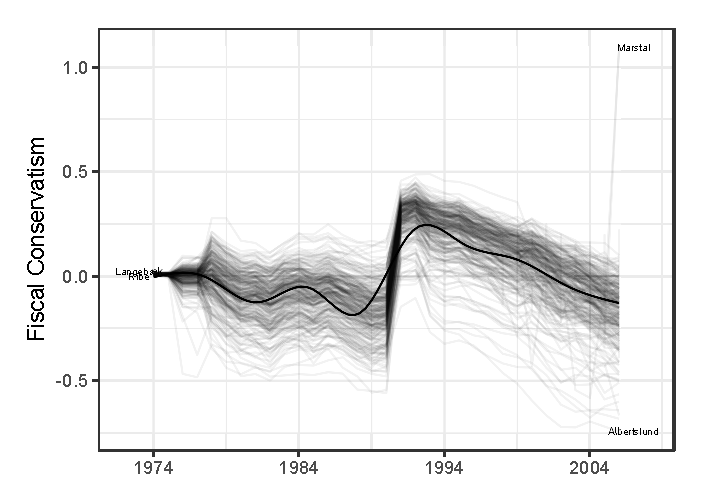
\includegraphics[scale = .85]{times_lines_inflation_adjusted.eps}
	\caption{\textbf{.}} \fnote{\emph{Note: .}}
	\label{fig:PermTest}
\end{figure}


\begin{figure}[!htb]
	\centering
	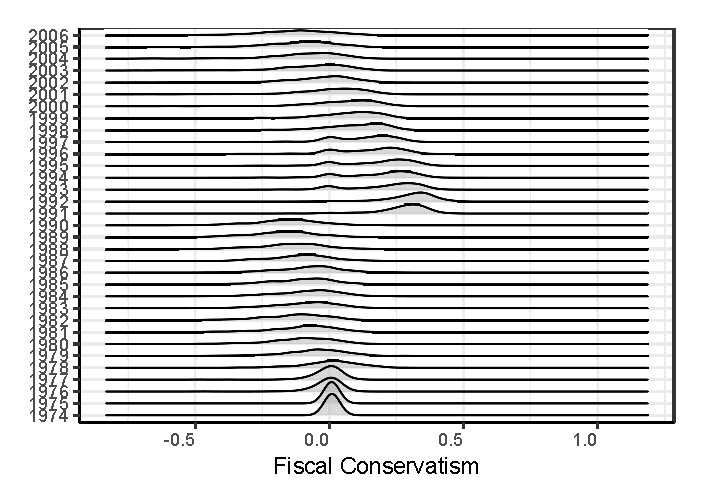
\includegraphics[scale = .85]{JoyPlotFiscal_inflation_adjusted.eps}
	\caption{\textbf{.}} \fnote{\emph{Note: .}}
	\label{fig:PermTest}
\end{figure}

\begin{landscape}
	\begin{figure}[!htb]
		\centering
		\includegraphics[scale = .85]{Map_of_FiscCon.eps}
		\caption{\textbf{.}} \fnote{\emph{Note: .}}
		\label{fig:PermTest}
	\end{figure}
\end{landscape}


\section{Dynamic Responsiveness}

\subsection{Measuring Local Policy Preferences}

\subsection{Results}



\begin{figure}[h]
	\centering
	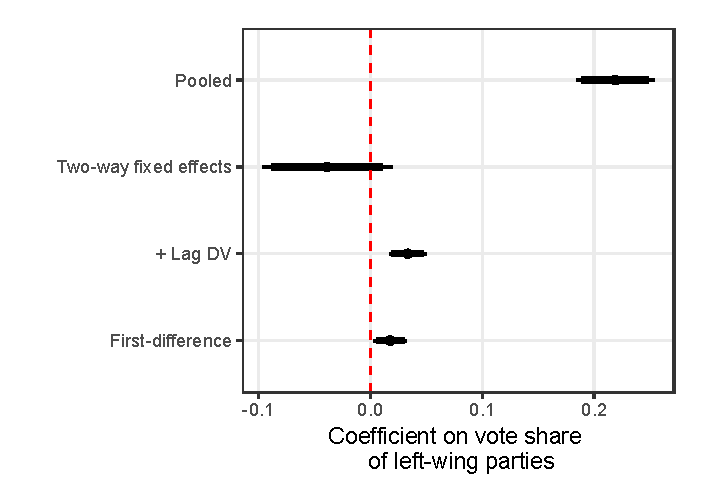
\includegraphics[scale = 1.1]{ggplot_coef_inflation_adjusted.eps}
	\caption{\textbf{Effect of Electoral Support for Right-wing Parties with a 4-year Lead.}} \fnote{\emph{Note: Point are unstandardized OLS coefficients. Lines are 90 pct. (thick) and 95 pct. (thin) confidence intervals computed using Arellano-White robust standard errors clustered at the municipality level, when no lags of the dependent variable are included. Beck-Katz panel-corrected standard errors used for dynamic models. Two and one lags of the dependent variable included, respectively, in the fixed effects and first-difference models.}}
	\label{fig:FourYearLead}
\end{figure}


\begin{figure}[h]
	\centering
	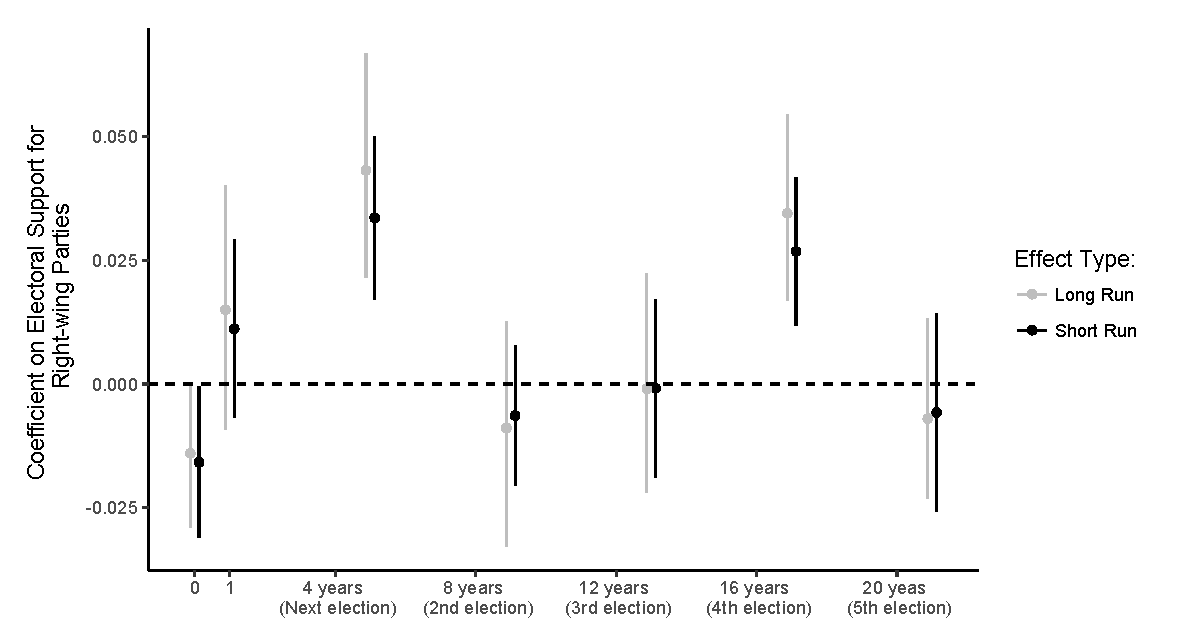
\includegraphics[scale = .8]{coef_on_varying_leads.eps}
	\caption{\textbf{Dynamic Effects of Public Mood.}} \fnote{\emph{Note: Black points represent the effect of electoral support for right-wing parties with different leads. Black lines are 95 pct. confidence intervals based on Arellano-White robust standard errors with municipal clustering. Grey points represent the additional long-run effect of electoral support for right-wing parties due to strong temporal autocorrelation in Fiscal Conservatism. Grey lines are 95 pct. confidence intervals computed from the relevant percentiles of a bootstrapped coefficient distribution based on 1,000 replications and resampling at the municipal level.}}
	\label{fig:LongRun}
\end{figure}



\section{The Effect of Governing Alone}

\subsection{A Regression Discontinuity in Policy Control}

\subsection{Results}

\begin{landscape}
	\begin{figure}[h]
		\centering
		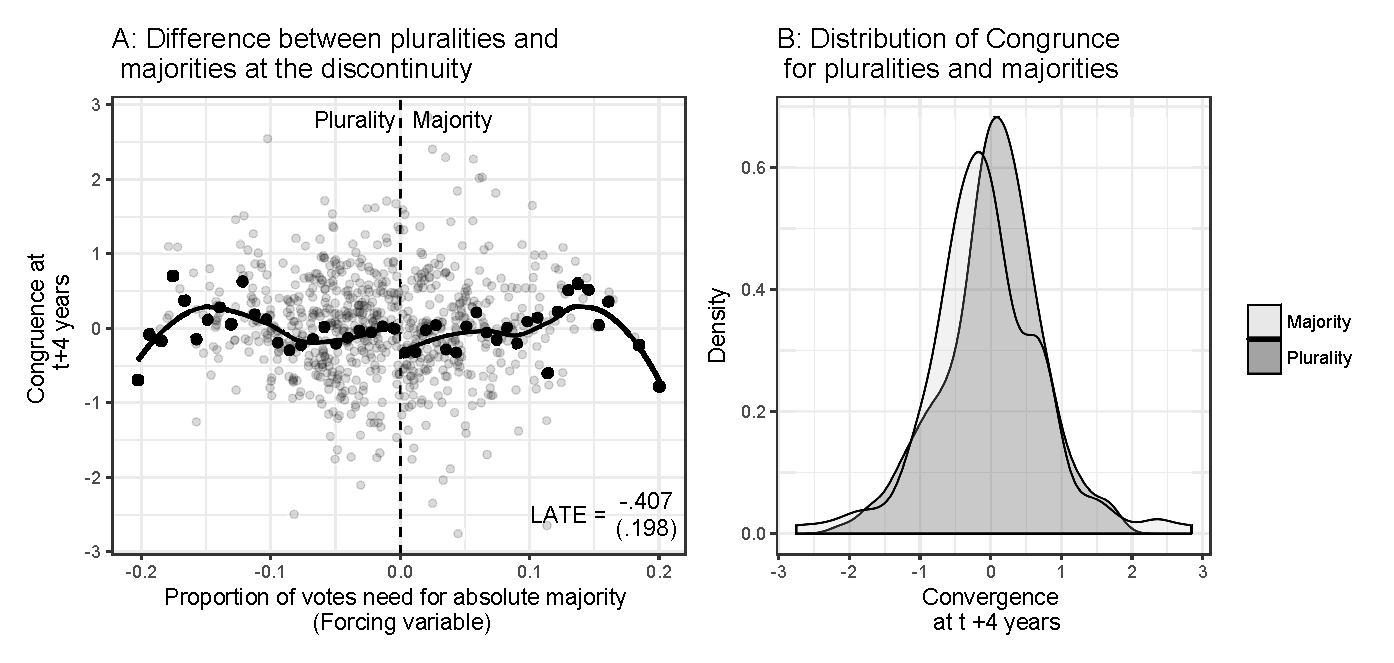
\includegraphics[scale = 1]{rddCongruence.eps}
		\caption{\textbf{.}} \fnote{\emph{Note: .}}
		\label{fig:PermTest}
	\end{figure}
\end{landscape}
	
\section{Conclusion}


\bibliographystyle{apa}
\bibliography{bibtex/library}


\beginsupplement

\section{Supplementary materials}

\subsection{S1. Descriptive Statistics}

	
\end{document}
